\documentclass{beamer}

\usepackage[T2A]{fontenc}
\usepackage[utf8]{inputenc}
\usepackage[english,russian]{babel}
\input{settings.tex}


\title{Аналитические решения}
\subtitle{Вычислительный интеллект, лекция 3}
\author{Сергей Савин}
\centering
\date{\mydate}



\begin{document}
\maketitle


%\begin{frame}{Content}
%
%\begin{itemize}
%\item Optimization problem
%\item Feasibility problem
%\item Norms and quadratic forms
%\item Problems with analytical solutions
%\item Weighted pseudoinverse
%\end{itemize}
%
%\end{frame}



\begin{frame}{Задача оптимизации}
	\begin{flushleft}
		
		Задача оптимизации имеет следующий вид:
		%
		\begin{equation}
			\begin{aligned}
				& \underset{\text{переменные решения}}{\text{minimize}}
				& & \text{целевая функция}, \\
				& \text{subject to}
				& & \text{ограничения}.
			\end{aligned}
		\end{equation}
		
		Решением задачи оптимизации является оптимальное значение переменных решения.
		
		\bigskip
		
		Например:
		%
		\begin{equation}
			\begin{aligned}
				& \underset{\bo{x}}{\text{minimize}}
				& & f(\bo{x}), \\
				& \text{subject to}
				& & \begin{cases}
					g(\bo{x}) = 0, \\
					h(\bo{x}) \leq 0.
				\end{cases}
			\end{aligned}
		\end{equation}
		
		В этом примере $\bo{x} \in \R^n$ — переменная решения, $f(\bo{x}): \ \R^n \rightarrow \R$ — целевая функция, $g(\bo{x}) = 0$ — ограничения-равенства, а $h(\bo{x}) \leq 0$ — ограничения-неравенства.
		
	\end{flushleft}
\end{frame}



\begin{frame}{Задача поиска допустимого решения}
	\begin{flushleft}
		
		Целевая функция всегда скалярна. Частным случаем целевой функции является константа:
		%
		\begin{equation}
			\begin{aligned}
				& \underset{\bo{x}}{\text{minimize}}
				& & 0, \\
				& \text{subject to}
				& & \begin{cases}
					g(\bo{x}) = 0, \\
					h(\bo{x}) \leq 0.
				\end{cases}
			\end{aligned}
		\end{equation}
		
		В этом случае любое $\bo{x}$, удовлетворяющее ограничениям, будет решением задачи. Такая задача называется \emph{задачей поиска допустимого решения}. Мы решали задачи такого типа, чтобы выяснить, существует ли какое-либо $\bo{x}$, удовлетворяющее ограничениям.
		
	\end{flushleft}
\end{frame}




\begin{frame}{Безусловная оптимизация}
	\begin{flushleft}
		
		Часто задача оптимизации не содержит ограничений:
		%
		\begin{equation}
			\begin{aligned}
				& \underset{\bo{x}}{\text{minimize}}
				& & f(\bo{x})
			\end{aligned}
		\end{equation}
		
		Мы можем назвать это \emph{безусловной оптимизацией}.
		
		\bigskip
		
		Обратите внимание, что переменная решения $\bo{x}$ может принадлежать множеству $\bo{x} \in \mathcal{X}$, или целевая функция может иметь область определения $f: \ \mathcal{D} \rightarrow \R$; в этих случаях множество допустимых значений $\bo{x}$, а также область определения функции представляют собой \emph{неявные} ограничения. 
		
		\bigskip
		
		Например, задача:
		
		$$\underset{x}{\text{minimize}} \ \ \ln x$$
		
		имеет неявное ограничение $x \geq 0$.
		
	\end{flushleft}
\end{frame}



\begin{frame}{Ограничения-равенства, Лагранжиан}
	\begin{flushleft}
		
		Рассмотрим задачи оптимизации с ограничениями-равенствами:
		%
		\begin{equation}
			\begin{aligned}
				& \underset{\bo{x}}{\text{minimize}}
				& & f(\bo{x}), \\
				& \text{subject to}
				& & g(\bo{x}) = 0
			\end{aligned}
		\end{equation}
		
		Мы решаем их, строя \emph{Лагранжиан}:
		
		\begin{equation}
			L(\bo{x}, \lambda) = f(\bo{x}) + \lambda\T g(\bo{x})
		\end{equation}
		
		Решение исходной задачи соответствует экстремуму Лагранжиана:
		%
		\begin{align}
			\frac{\partial L(\bo{x}, \lambda)}{\partial \bo{x}} = 0
			\\
			\frac{\partial L(\bo{x}, \lambda)}{\partial \lambda} = 0
		\end{align}
		
	\end{flushleft}
\end{frame}



\begin{frame}{Примеры безусловной оптимизации}
	\begin{flushleft}
		
		
		Некоторые типы задач оптимизации допускают аналитическое решение. Например:
		
		
		Задача 1. $\text{minimize} \ ||\mathbf{x}||$. \textcolor{white}{Решение $\mathbf{x} = \mathbf{0}$} 
		
		\bigskip
		
		Задача 2. $\text{minimize} \ ||\mathbf{A}\mathbf{x}||$. \textcolor{white}{Решение $\mathbf{x} = \mathbf{0}$.}
		
		\bigskip
		
		Задача 3. $\text{minimize} \ ||\mathbf{A}\mathbf{x} + \mathbf{b}||$. 
		
		\bigskip
		
		Нам известно решение задачи $\textcolor{mydarkgray}{\text{minimize} \ ||\mathbf{A}\mathbf{x} - \mathbf{b}||}$, которым является $\mathbf{x} = \mathbf{A}^+ \mathbf{b}$. Следовательно, задача 3 имеет решение $\mathbf{x} = -\mathbf{A}^+ \mathbf{b}$.
		
	\end{flushleft}
\end{frame}



\begin{frame}{МНК с ограничениями}
	\begin{flushleft}
		
		
		Задача 4. (форма 1)
		%
		\begin{equation}
			\begin{aligned}
				& \underset{\mathbf{x}}{\text{minimize}}
				& & || \mathbf{x} ||, \\
				& \text{subject to}
				& & \mathbf{A} \mathbf{x} = \mathbf{b}.
			\end{aligned}
		\end{equation}
		
		
		Все решения $\mathbf{A} \mathbf{x} = \mathbf{b}$ записываются как $\mathbf{x} = \mathbf{A}^+\mathbf{b} + \mathbf{N}\mathbf{z}$, где $\mathbf{N} = \text{null}(\mathbf{A})$. 
		
		\bigskip
		
		Поскольку решение из нуль-пространства $\mathbf{N}\mathbf{z}$ и частное решение $\mathbf{A}^+\mathbf{b}$ ортогональны, решение с минимальной нормой соответствует $\mathbf{z} = \mathbf{0}$, следовательно:
		
		\begin{equation}
			\mathbf{x} = \mathbf{A}^+\mathbf{b}
		\end{equation}
		
	\end{flushleft}
\end{frame}

\begin{frame}{МНК с ограничениями}
	\begin{flushleft}
		
		
		Таким образом, решением является $\mathbf{x} = \mathbf{A}^+\mathbf{b}$. Обратите внимание, что решения для задач 3 и 4 записываются одинаково (если не учитывать знак), хотя в задаче 3 требуется минимизировать невязку линейной системы, а в задаче 4 — найти решение с минимальной нормой. 
		
		\bigskip
		
		Это иллюстрирует важный факт: решение задачи наименьших квадратов, сформулированной либо как «минимизация невязки», либо как «решение с минимальной нормой», задается одной и той же формулой, которую мы называем псевдообратной матрицей Мура — Пенроуза.
		
		
	\end{flushleft}
\end{frame}


\begin{frame}{МНК с ограничениями}
	\begin{flushleft}
		
		
		Задача 4. (форма 2)
		%
		\begin{equation}
			\begin{aligned}
				& \underset{\mathbf{x}}{\text{minimize}}
				& & \frac{1}{2} \bo{x}\T \bo{x}, \\
				& \text{subject to}
				& & \bo{A} \bo{x} = \bo{b}.
			\end{aligned}
		\end{equation}
		
		Найдем Лагранжиан $L =\frac{1}{2} \bo{x}\T \bo{x} + \lambda\T ( \mathbf{A} \mathbf{x} - \bo{b})$. Решение исходной задачи соответствует его экстремуму:
		
		\begin{align}
			\frac{\partial L}{\partial \bo{x}} &=  \bo{x} + \bo{A}\T  \lambda = 0 
			\\
			\frac{\partial L}{\partial \lambda} &=  \bo{A} \bo{x}- \bo{b} = 0
		\end{align}
		
		Мы можем выразить $\bo{x} = -\bo{A}\T  \lambda$ и подставить: $-\bo{A} \bo{A}\T  \lambda= \bo{b}$. Если $\text{det}(\bo{A} \bo{A}\T ) \neq 0$, то:
		%
		\begin{align}
			\lambda &= - (\bo{A} \bo{A}\T )^{-1} \bo{b}
			\\
			\bo{x} &= \bo{A}\T  (\bo{A} \bo{A}\T )^{-1} \bo{b} =  \mathbf{A}^+\mathbf{b} \ \ \ \textcolor{mygray}{\text{правое обратное}}
		\end{align}		
		
	\end{flushleft}
\end{frame}




\begin{frame}{Взвешенное МНК с ограничениями}
	\begin{flushleft}
		
		Задача 5. Рассмотрим задачу о взвешенном псевдообратном операторе:
		%
		\begin{equation}
			\begin{aligned}
				& \underset{\bo{x}}{\text{minimize}}
				& & \bo{x}\T \bo{W} \bo{x}, \\
				& \text{subject to}
				& & \bo{A}\bo{x}=\bo{b}
			\end{aligned}
		\end{equation}
		
		Мы можем использовать множители Лагранжа, чтобы переписать задачу как минимизацию функции $L(\bo{x}, \lambda) = \bo{x}\T \bo{W} \bo{x} + \lambda\T ( \bo{A}\bo{x}-\bo{b})$; условия оптимальности означают, что $\frac{\partial L}{\partial  \bo{x}} = 0$ и $\frac{\partial  L}{\partial  \lambda} = \bo{A}\bo{x}-\bo{b} = 0$, следовательно:
		%
		\begin{align}
			2\bo{x}\T \bo{W} + \lambda\T \bo{A} = 0
		\end{align}		
		
		Отсюда $\bo{x} = -\frac{1}{2} \bo{W}^{-1} \bo{A}\T \lambda$, а поскольку $\bo{A}\bo{x}-\bo{b} = 0$, получаем:
		%
		\begin{align}
			-\frac{1}{2}\bo{A}\bo{W}^{-1} \bo{A}\T \lambda= \bo{b} \\
			\lambda = -2 (\bo{A}\bo{W}^{-1} \bo{A}\T)^{-1} \bo{b} \\
			\bo{x} = \bo{W}^{-1} \bo{A}\T (\bo{A}\bo{W}^{-1} \bo{A}\T)^{-1} \bo{b}
		\end{align}		
		
		
	\end{flushleft}
\end{frame}



\begin{frame}{Взвешенное МНК со смещением, 1}
	\begin{flushleft}
		
		Задача 6. Рассмотрим задачу о взвешенном псевдообратном операторе (где $\bo{H} = \bo{H}\T > 0$):
		%
		\begin{equation}
			\begin{aligned}
				& \underset{\bo{x}}{\text{minimize}}
				& & \frac{1}{2} \bo{x}\T \bo{H} \bo{x} + \bo{f}\T \bo{x} , \\
				& \text{subject to}
				& & \bo{A}\bo{x}=\bo{b}
			\end{aligned}
		\end{equation}
		%
		Лагранжиан для этой задачи имеет вид:
		%
		\begin{align}
			L = \frac{1}{2} \bo{x}\T \bo{H} \bo{x} + \bo{f}\T \bo{x} + \lambda\T (\bo{A}\bo{x}-\bo{b})
		\end{align}
		%
		Приравнивая частные производные к нулю, получаем:
		%
		\begin{align}
			\frac{\partial L}{\partial \bo{x}} &=
			\bo{x}\T \bo{H}  + \bo{f}\T + \lambda\T \bo{A} = 0 
			\\
			\frac{\partial L}{\partial \lambda} &= \bo{A}\bo{x}-\bo{b} = 0
		\end{align}		
		%
		Из первого уравнения получаем $\bo{x}  = -\bo{H}^{-1}(\bo{f} + \bo{A}\T \lambda)$
		
	\end{flushleft}
\end{frame}

\begin{frame}{Взвешенное МНК со смещением, 2}
	\begin{flushleft}
		
		Из $\bo{A}\bo{x}=\bo{b}$ и $\bo{x}  = -\bo{H}^{-1}(\bo{f} + \bo{A}\T \lambda)$ получаем:
		%
		\begin{align}
			-\bo{A}\bo{H}^{-1}(\bo{f} + \bo{A}\T \lambda)=&\bo{b}
			\\
			-\bo{A}\bo{H}^{-1} \bo{A}\T \lambda = &\bo{b} + \bo{A}\bo{H}^{-1}\bo{f}
			\\
			\lambda = -(\bo{A}\bo{H}^{-1} \bo{A}\T)^{-1}(&\bo{b} + \bo{A}\bo{H}^{-1}\bo{f})
		\end{align}		
		%
		Подставляем обратно $\bo{x}$: 
		%
		\begin{align}
			\bo{x}  &= -\bo{H}^{-1}(\bo{f} - \bo{A}\T (\bo{A}\bo{H}^{-1} \bo{A}\T)^{-1}(\bo{b} + \bo{A}\bo{H}^{-1}\bo{f}))
			\\
			\bo{x}  &= \bo{H}^{-1}(\bo{A}\T (\bo{A}\bo{H}^{-1} \bo{A}\T)^{-1} \bo{A}\bo{H}^{-1}-\bo{I})\bo{f}
			+ \\ &+
			\bo{H}^{-1} (\bo{A}\T (\bo{A}\bo{H}^{-1} \bo{A}\T)^{-1} \bo{b} 
		\end{align}		
		
		
	\end{flushleft}
\end{frame}




\begin{frame}{Взвешенное МНК со смещением, 3}
	\begin{flushleft}
		
		Целевая функция $f(\bo{x}) = \frac{1}{2} \bo{x}\T \bo{H} \bo{x} + \bo{f}\T \bo{x}$ может быть преобразована с помощью следующей замены переменных:
		%
		\begin{align}
			\bo{z} = \bo{x} + \bo{H}^{-1}\bo{f}, \ \ \ \bo{x} = \bo{z} - \bo{H}^{-1}\bo{f}.
		\end{align}
		%
		таким образом, получаем:
		%
		\begin{align*}
			f(\bo{z}) &= \frac{1}{2} (\bo{z} - \bo{H}^{-1}\bo{f})\T \bo{H} (\bo{z} - \bo{H}^{-1}\bo{f}) + \bo{f}\T (\bo{z} - \bo{H}^{-1}\bo{f})
			\\
			&= \frac{1}{2} \bo{z}\T \bo{H} \bo{z} - 
			\textcolor{myblue}{\bo{z}\T \bo{H} \bo{H}^{-1}\bo{f}} + 
			\textcolor{mydarkgreen}{\frac{1}{2} \bo{f}\T \bo{H}^{-1}\bo{H} \bo{H}^{-1}\bo{f}} + 
			\textcolor{myblue}{\bo{f}\T \bo{z}} - \textcolor{mydarkgreen}{\bo{f}\T\bo{H}^{-1}\bo{f}} =
			\\
			&= \frac{1}{2} \bo{z}\T \bo{H} \bo{z}  - \frac{1}{2} \bo{f}\T \bo{H}^{-1}\bo{f}
		\end{align*}
		
		Поскольку $ \frac{1}{2} \bo{f}\T \bo{H}^{-1}\bo{f}$ является константой, минимизация $f(\bo{z})$ эквивалентна минимизации $f^*(\bo{z})$:
		%
		\begin{align*}
			f^*(\bo{z}) =  \frac{1}{2} \bo{z}\T \bo{H} \bo{z}
		\end{align*}
		
		Это позволяет нам свести Задачу 6 к Задаче 5.
		
		
	\end{flushleft}
\end{frame}




\begin{frame}{МНК со свободными переменными, 1}
	\begin{flushleft}
		
		Задача 7. Рассмотрим модификацию задачи взвешенных наименьших квадратов:
		%
		\begin{equation}
			\begin{aligned}
				& \underset{\bo{x}, \bo{y}}{\text{minimize}}
				& & \frac{1}{2} \bo{x}\T \bo{x}, \\
				& \text{subject to}
				& & \bo{A}\bo{x} + \bo{B}\bo{y}=\bo{c}
			\end{aligned}
		\end{equation}
		%
		Лагранжиан для этой задачи:
		%
		\begin{align}
			L = \frac{1}{2} \bo{x}\T \bo{x} + \lambda\T ( \bo{A}\bo{x} + \bo{B}\bo{y}-\bo{c})
		\end{align}
		%
		Приравнивая частные производные к нулю, получаем:
		%
		\begin{align}
			\frac{\partial L}{\partial \bo{x}} &=
			\bo{x} + \bo{A}\T \lambda = 0 
			\\
			\frac{\partial L}{\partial \bo{y}} &=
			\bo{B}\T \lambda = 0 
			\\
			\frac{\partial L}{\partial \lambda} &= \bo{A}\bo{x} + \bo{B}\bo{y}-\bo{c} = 0
		\end{align}		
		
		
	\end{flushleft}
\end{frame}



\begin{frame}{МНК со свободными переменными, 2}
	\begin{flushleft}
		
		
		Мы можем решить это как систему:
		%
		\begin{align}
			\begin{bmatrix}
				\bo{x}\\ \bo{y} \\ \lambda
			\end{bmatrix}
			=
			\begin{bmatrix}
				\bo{I} & \bo{0} & \bo{A}\T \\
				\bo{0} & \bo{0} & \bo{B}\T \\
				\bo{A} & \bo{B} & \bo{0}
			\end{bmatrix}^+
			\begin{bmatrix}
				\bo{0}\\ \bo{0} \\ \bo{c} 
			\end{bmatrix}
		\end{align}		
		
		
		
	\end{flushleft}
\end{frame}




\begin{frame}{Пример, 1}
	\begin{flushleft}
		
		Квадрокоптер летит вдоль прямой, заданной точкой $\bo{c}$ и направлением $\bo{v}$. Найдите точку, в которой он пролетит ближе всего к наземной станции, расположенной в точке $\bo{a}$.
		
		\bigskip
		
		\emph{Решение}. Любую точку на прямой можно описать как $\bo{x} = \bo{v} \xi + \bo{c}$. Таким образом, задачу можно записать в виде:
		%
		\begin{equation}
			\begin{aligned}
				& \underset{\bo{x}, \alpha}{\text{minimize}}
				& & \frac{1}{2}(\bo{x}- \bo{a})\T(\bo{x}- \bo{a}), \\
				& \text{subject to}
				& & \bo{x} = \bo{v} \xi + \bo{c}
			\end{aligned}
		\end{equation}
		
		Лагранжиан задачи:
		%
		\begin{equation}
			L =  \frac{1}{2}(\bo{x}- \bo{a})\T(\bo{x}- \bo{a}) + \lambda\T  ( \bo{v} \xi + \bo{c} - \bo{x})
		\end{equation}
		
		
		
	\end{flushleft}
\end{frame}



\begin{frame}{Пример, 2}
	\begin{flushleft}
		
		\begin{equation}
			L =  \frac{1}{2}(\bo{x}- \bo{a})\T(\bo{x}- \bo{a}) + \lambda\T ( \bo{v} \xi + \bo{c} - \bo{x})
		\end{equation}
		
		Частные производные Лагранжиана:
		
		\begin{align}
			\frac{\partial L}{\partial \bo{x}} &=  (\bo{x}- \bo{a}) - \lambda = 0
			\\
			\frac{\partial L}{\partial \alpha} &=  \lambda\T \bo{v} = 0
			\\
			\frac{\partial L}{\partial  \lambda} &=   \bo{v} \xi + \bo{c} - \bo{x} = 0
		\end{align}
		
		Это можно выразить как:
		
		\begin{align}
			\begin{bmatrix}
				\bo{I} & 0 & -\bo{I} 
				\\
				0 & 0 & \bo{v}\T
				\\
				-\bo{I} & \bo{v} & 0
			\end{bmatrix}
			\begin{bmatrix}
				\bo{x} \\ \xi \\  \lambda
			\end{bmatrix}
			=
			\begin{bmatrix}
				\bo{a} \\ 0 \\  -\bo{c}
			\end{bmatrix}
		\end{align}
		
		что можно решить с помощью обращения матрицы.
		
	\end{flushleft}
\end{frame}



\begin{frame}{Пример, 3}
	\begin{flushleft}
		
		Используя уравнения $\textcolor{myred}{\bo{x}- \bo{a} = \lambda}$ и $\textcolor{myblue}{\lambda\T \bo{v} = 0}$ и $\textcolor{mydarkgreen}{\bo{v} \xi + \bo{c} = \bo{x}}$ мы можем записать:
		
		\begin{align}
			\bo{v}\T (\bo{x}- \bo{a}) = 0
			\\
			\bo{v}\T \bo{v} \xi + \bo{v}\T\bo{c} - \bo{v}\T \bo{a} = 0
		\end{align}
		
		Поскольку $\bo{v}\T \bo{v} = 1$, то $\xi  = \bo{v}\T (\bo{a} - \bo{c})$. Следовательно:
		
		\begin{align}
			\bo{x} &= \bo{v} \bo{v}\T \bo{a} + (\bo{I} - \bo{v} \bo{v}\T) \bo{c}
			\\
			\lambda &= (\bo{I} - \bo{v} \bo{v}\T)(\bo{c} - \bo{a})
		\end{align}
		
		
	\end{flushleft}
\end{frame}



\begin{frame}{Пример, 4}
	\begin{flushleft}
		
		% TODO: \usepackage{graphicx} required
		\begin{figure}
			\centering
			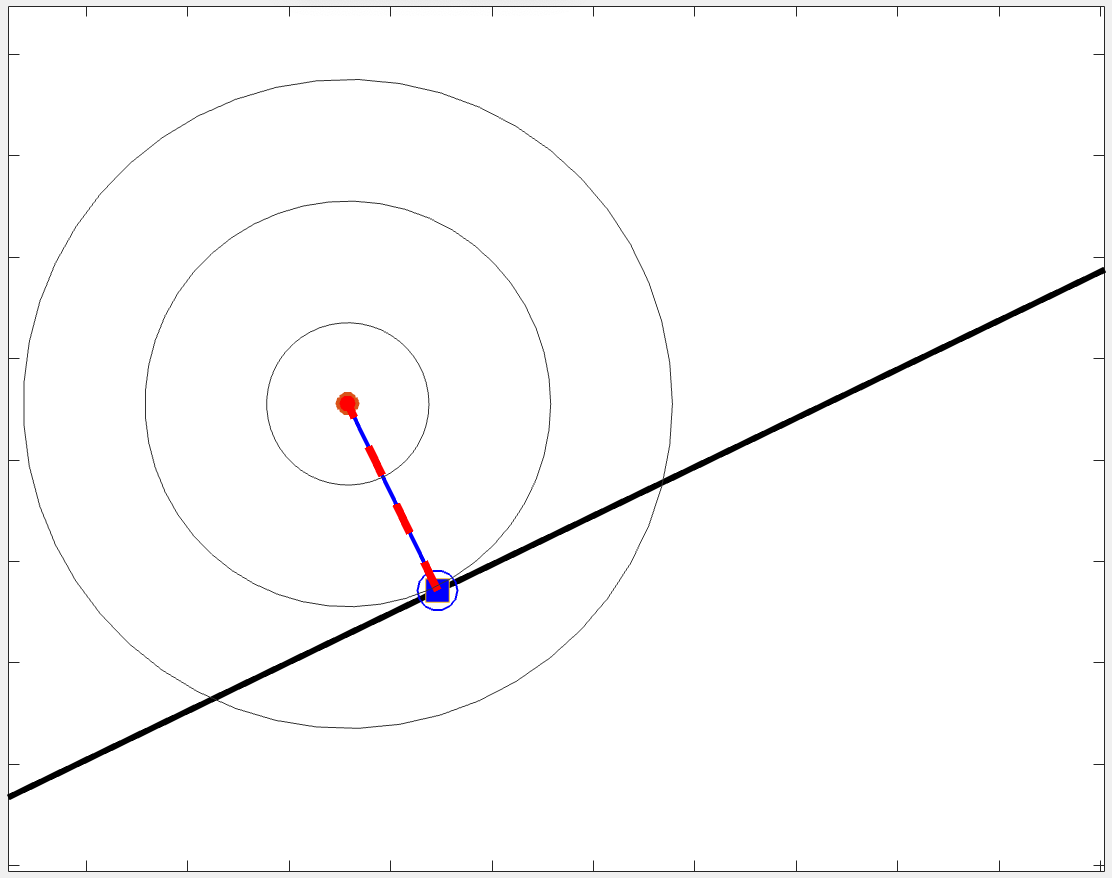
\includegraphics[width=0.7\linewidth]{fig1}
			\caption{Иллюстрация к задаче}
		\end{figure}
		
		
		
	\end{flushleft}
\end{frame}






\myqrframe


\begin{frame}{Right inverse and SVD}
	\begin{flushleft}
		
		We can prove that $ \bo{A}\T  (\bo{A} \bo{A}\T )^{-1} = \bo{A}^+$.
		
		\bigskip
		
		We can re-write the expression $\bo{A} \bo{A}\T  \lambda= -\bo{b}$ using compact (reduced) SVD decomposition $\bo{A} = \bo{C}\Sigma\bo{R}\T$ (here $\bo{C}$ is the the orthonormal basis in the column space of $\bo{A}$, $\bo{R}$ is the orthonormal basis in the row space of $\bo{A}$):
		%
		\begin{align}
			\bo{C}\Sigma\bo{R}\T \bo{R}\Sigma\bo{C}\T  \lambda= -\bo{b}
			\\
			\bo{C}\Sigma \Sigma\bo{C}\T  \lambda= -\bo{b}
			\\
			\textcolor{mydarkred}{\bo{C}\T  \lambda}= -\Sigma^{-2} \bo{C}\T \bo{b}
		\end{align}				
		%
		Next, we do the same with $\bo{x} = -\bo{A}\T  \lambda$:
		%
		\begin{align}
			\bo{x} = -\bo{R}\Sigma\textcolor{mydarkred}{\bo{C}\T  \lambda}
			\\
			\bo{x} = \bo{R}\Sigma\Sigma^{-2} \bo{C}\T \bo{b}
			\\
			\bo{x} = \bo{R}\Sigma^{-1} \bo{C}\T \bo{b}
		\end{align}				
		%
		But $ \bo{R}\Sigma^{-1} \bo{C}\T \ = \bo{A}^+$, so $\bo{x} =\bo{A}^+ \bo{b}$. 
		
	\end{flushleft}
\end{frame}


\begin{frame}{Problem 4. Solution via orthogonality}
	\begin{flushleft}
		
		\begin{small}
		\begin{equation}
			\begin{aligned}
				& \underset{\mathbf{x}}{\text{minimize}}
				& & \frac{1}{2} \bo{x}\T \bo{x}, \\
				& \text{subject to}
				& & \bo{A} \bo{x} = \bo{b}.
			\end{aligned}
		\end{equation}
		
		All solutions to $\bo{A} \bo{x} = \bo{b}$ are written as $\bo{x} = \bo{A}^+\bo{b} + \bo{N}\bo{z}$, where $\bo{N} = \text{null}(\bo{A})$, and $\bo{A}^+\bo{b} \in \text{row}(\bo{A})$ as we proved previously.  The cost function is:
		%
		\begin{align}
			f_c &= \frac{1}{2} (\bo{A}^+\bo{b} + \bo{N}\bo{z})\T (\bo{A}^+\bo{b} + \bo{N}\bo{z}) 
		\end{align}
		%
		We find extremum:
		%
		\begin{align}
			\frac{\partial f_c}{\partial \bo{z}} &= \bo{N}\T \bo{A}^+\bo{b} + \bo{N}\T\bo{N}\bo{z} = 0
			\\
			\bo{z} &= - \bo{N}\T \bo{A}^+\bo{b} 
			\\
			\bo{x} &= \bo{A}^+\bo{b} -  \bo{N}\bo{N}\T \bo{A}^+\bo{b} 
		\end{align}
		
		Columns of $\bo{A}^+$ lie in the row space of $\bo{A}$, so $\bo{N}\T \bo{A}^+ = 0$:
		%
		\begin{align}
			\bo{x} &= \bo{A}^+\bo{b}
		\end{align}
	\end{small}
		
	\end{flushleft}
\end{frame}



\begin{frame}{Problems with weighted norm}
	\begin{flushleft}
		
		Problem 5. 
		%
		\begin{equation}
			\begin{aligned}
				& \underset{\mathbf{x}}{\text{minimize}}
				& & || \mathbf{D}\mathbf{x} ||, \\
				& \text{subject to}
				& & \mathbf{A} \mathbf{x} = \mathbf{b}.
			\end{aligned}
		\end{equation}
		
		One way to think about it is to first find all solution to the constraint equation $\mathbf{A} \mathbf{x} = \mathbf{b}$ and then find optimal one among them. As we know, all solutions are given as: $\mathbf{x} = \mathbf{A}^+\mathbf{b} + \mathbf{N}\mathbf{z}$, where $\mathbf{N} = \text{null}(\mathbf{A})$. Then our cost function becomes: $|| \mathbf{D}\mathbf{A}^+\mathbf{b} +  \mathbf{D}\mathbf{N}\mathbf{z} ||$, which is equivalent to the problem 3. Thus, we can write solution as: 
		$\mathbf{z}^* = -(\mathbf{D}\mathbf{N})^+ \mathbf{D}\mathbf{A}^+\mathbf{b}$. In terms of $\mathbf{x}$ solution is:
		
		\begin{equation}
			\mathbf{x}^* = \mathbf{A}^+\mathbf{b}-\mathbf{N}(\mathbf{D}\mathbf{N})^+ \mathbf{D}\mathbf{A}^+\mathbf{b}
		\end{equation}
		\begin{equation}
			\mathbf{x}^* =( \mathbf{I}-\mathbf{N}(\mathbf{D}\mathbf{N})^+ \mathbf{D})\mathbf{A}^+\mathbf{b}
		\end{equation}
		
	\end{flushleft}
\end{frame}



\begin{frame}{Problems with weighted norm}
	\begin{flushleft}
		
		Problem 6. 
		%
		\begin{equation}
			\begin{aligned}
				& \underset{\mathbf{x}}{\text{minimize}}
				& & || \mathbf{D}\mathbf{x} + \mathbf{f} ||, \\
				& \text{subject to}
				& & \mathbf{A} \mathbf{x} = \mathbf{b}.
			\end{aligned}
		\end{equation}
		
		After the same initial step, we arrive at the cost function $|| \mathbf{D}\mathbf{N}\mathbf{z} + \mathbf{D}\mathbf{A}^+\mathbf{b} + \mathbf{f}||$. It is only different in the constant term, and the solution is found as follows:
		
		
		\begin{equation}
			\mathbf{z}^* = -(\mathbf{D}\mathbf{N})^+ (\mathbf{D}\mathbf{A}^+\mathbf{b} + \mathbf{f})
		\end{equation}
		\begin{equation}
			\mathbf{x}^* = \mathbf{A}^+\mathbf{b}-\mathbf{N}(\mathbf{D}\mathbf{N})^+ (\mathbf{D}\mathbf{A}^+\mathbf{b} + \mathbf{f})
		\end{equation}
		
		
	\end{flushleft}
\end{frame}




\begin{frame}{Positive-definite matrices}
	\begin{flushleft}
		
		A symmetric positive-definite matrix $\bo{M}$ has the following properties:
		
		\begin{align}
			&\bo{M} = \bo{M}\T
			\\
			&\bo{x}\T \bo{M} \bo{x} > 0, \ \ \forall \bo{x} \neq 0
			\\
			& \text{det}(\bo{M}) \neq 0
		\end{align}
		
		Positive-definite matrices (with non-repeating eigenvalues) have orthogonal eigenvectors, making their eigenbasis orthonormal:
		
		\begin{align}
			& \bo{M} \bo{V} = \bo{V} \Lambda  
			\\
			& \bo{M} = \bo{V} \Lambda \bo{V}\T 
		\end{align}
		
	\end{flushleft}
\end{frame}




\begin{frame}{Matrix square root}
	\begin{flushleft}
		
		For a symmetric positive-definite matrix $\bo{M}$ we can define a square root:
		
		\begin{align}
			\bo{M} &= \sqrt{\bo{M} } \sqrt{\bo{M} }
			\\
			\bo{M} &= \bo{M}^\frac{1}{2} \bo{M}^\frac{1}{2}
		\end{align}
		
		We can find a square root via eigendecomposition:
		
		\begin{align}
			& \bo{M} = \bo{V} \Lambda \bo{V}\T 
			\\
			&  \Lambda =  \bo{F} \bo{F}
			\\
			& \bo{M} = \bo{V} \bo{F} \bo{F} \bo{V}\T 
			\\
			& \bo{M} = \bo{V} \bo{F} \bo{V}\T\bo{V}  \bo{F} \bo{V}\T 
			\\
			& \sqrt{\bo{M} }  = \bo{V} \bo{F} \bo{V}\T
			\\
			&\bo{M} = \sqrt{\bo{M} } \sqrt{\bo{M} } 
		\end{align}
		
		
		
	\end{flushleft}
\end{frame}




\begin{frame}{Problems quadratic cost}
	\begin{flushleft}
		
		Problem 7. 
		%
		\begin{equation}
			\begin{aligned}
				& \underset{\mathbf{x}}{\text{minimize}}
				& & \mathbf{x}^\top \mathbf{H} \mathbf{x} + \mathbf{c}^\top\mathbf{x}, \\
				& \text{subject to}
				& & \mathbf{A} \mathbf{x} = \mathbf{b}.
			\end{aligned}
		\end{equation}
		
		where $\mathbf{H}$ is positive-definite.
		
		\bigskip
		
		Assume that we found a decomposition $\mathbf{H} = \mathbf{D}^\top\mathbf{D}$. We can also find such $\mathbf{f}$ that $2\mathbf{f}^\top\mathbf{D} = \mathbf{c}^\top$. Then our cost function becomes $\mathbf{x}^\top \mathbf{D}^\top\mathbf{D} \mathbf{x} + 2\mathbf{f}^\top\mathbf{D}\mathbf{x}$, which as we saw before has coinciding minimum with the cost function $||\mathbf{D}\mathbf{x} + \mathbf{f}||$.
		
		\bigskip
		
		Therefore the problem has the same solution as Problem 5, after the mentioned above change in constants.
		
	\end{flushleft}
\end{frame}



\begin{frame}{Weighted pseudoinverse, unconstrained type}
	\begin{flushleft}
		
		Consider a weighted pseudoinverse problem:
		%
		\begin{align}
			\text{minimize} \ \ ||\bo{A}\bo{x}-\bo{b}||_\bo{W}
		\end{align}		
		%
		where $||\bo{x}||_\bo{W} = \sqrt{\bo{x}\T\bo{W}\bo{x}}$ and $\bo{W} > 0$. We can re-write the problem as:
		%
		\begin{align}
			\text{minimize} \ \ (\bo{A}\bo{x}-\bo{b})\T\bo{W}^\frac{1}{2}\bo{W}^\frac{1}{2}(\bo{A}\bo{x}-\bo{b})
		\end{align}
		
		But this is the same as solving least-squares problem for equality $\bo{W}^\frac{1}{2}\bo{A}\bo{x}=\bo{W}^\frac{1}{2}\bo{b}$, which is does via Moore-Penrose pseudoinverse:
		%
		\begin{align}
			\bo{x}=(\bo{W}^\frac{1}{2}\bo{A})^+\bo{W}^\frac{1}{2}\bo{b}
		\end{align}
		
	\end{flushleft}
\end{frame}


\end{document}
